\section{Boundary spectra in the open central gaps}
\label{v11:sec:gap-limits}

Retain $\mathscr U,\mathscr C_\pm,L_b,H_b$ from
Section~\ref{v11:sec:phase-constants}. The same localization determines
every limiting eigenvalue away from zero and the band edges. Put
\[
 \Sigma=\{0\}\cup[-1,-g]\cup[g,1],\qquad
 \Omega=\mathbb C\setminus\Sigma,\qquad g=2^{-1/2}.
\]

\begin{lemma}[The reference resolvent gap]\label{v11:lem:model-gap}
The spectra of $\mathscr C_m,\mathscr C_+,\mathscr C_-$ are contained
in $\Sigma$.  The finite model has exactly $m$ positive and $m$ negative
eigenvalues.  Their resolvents, and the translated right resolvents,
converge strongly to the appropriate half-line resolvents, including
their adjoints, uniformly on compact subsets of $\Omega$.
\end{lemma}
\begin{proof}
For a finite or either half-infinite cell projection $E$, the scalar
compressions $C_E=E\mathcal L(c)E$ and $S_E=E\mathcal L(s)E$ satisfy
$C_E+S_E\ge I$ on that cell space because
$c(\theta)+s(\theta)\ge1$.  Hence
\[
 C_E^2+S_E^2
 =\tfrac12[(C_E+S_E)^2+(C_E-S_E)^2]\ge\tfrac12I.
\]
The row operator $B_E=(S_E,C_E)$ has $B_EB_E^*\ge I/2$ and is onto.
The polar decomposition of the star operator
$\left(\begin{smallmatrix}0&B_E\\B_E^*&0\end{smallmatrix}\right)$
therefore confines its nonzero spectrum to the two bands.  Its norm is
at most one by compression of $\mathcal L(a)$; the ambient complement
adds only zero.  The finite count follows from the row rank $m$.

At each fixed boundary the finite compressions converge strongly.
Continuous functional calculus on the common spectral set $\Sigma$
gives strong resolvent convergence. On compact $K\subset\Omega$ the
norm bound $\operatorname{dist}(K,\Sigma)^{-1}$, the resolvent identity
and finite nets give uniformity; conjugating the parameter handles
adjoints.
\end{proof}

For fixed real $l,h$ let $E_m=P_{(l,m+h)}$ in physical coordinates and
define
\[
 \mathscr A_m(l,h)=\mathscr U^*E_m\mathcal G E_m\mathscr U,
 \quad
 \mathscr A_l^+=\mathscr U^*L_l\mathcal G L_l\mathscr U,
 \quad
 \mathscr A_h^-=\mathscr U^*H_h\mathcal G H_h\mathscr U,
\]
\[
 D_l^+=\mathscr A_l^+-\mathscr C_+,
 \qquad D_h^-=\mathscr A_h^--\mathscr C_-.
\]
The last two differences are trace class.  Adding the gauge and strip
localizations gives
\begin{equation}\label{v11:eq:combined-gap-localization}
 \|\mathscr A_m(l,h)-\mathscr C_m-D_l^+
                  -\mathsf S^mD_h^-\mathsf S^{-m}\|_1\to0.
\end{equation}
Combining the corrections before taking the resolvent is essential:
the star baseline has a proved gap, whereas a physical half-line
baseline could itself have a gap eigenvalue.

Define, for $\lambda\in\Omega$,
\begin{align}
 F_m(\lambda;l,h)
   &=\det\bigl[I+(\mathscr A_m(l,h)-\mathscr C_m)
                             (\mathscr C_m-\lambda)^{-1}\bigr],\nonumber\\
 F_+(\lambda;l)
   &=\det\bigl[I+D_l^+(\mathscr C_+-\lambda)^{-1}\bigr],\qquad
 F_-(\lambda;h)
   =\det\bigl[I+D_h^-(\mathscr C_--\lambda)^{-1}\bigr].
 \label{v11:eq:gap-determinants}
\end{align}
They are analytic Fredholm determinants of identity plus trace-class
operators.  The signs follow from
$I+(A-C)(C-\lambda)^{-1}=(A-\lambda)(C-\lambda)^{-1}$.

\begin{theorem}[Local gap eigenvalue convergence]\label{v11:thm:gap-limits}
Locally uniformly on $\Omega$,
\begin{equation}\label{v11:eq:gap-det-limit}
 F_m(\lambda;l,h)\longrightarrow F_+(\lambda;l)F_-(\lambda;h).
\end{equation}
The two limiting factors have precisely the eigenvalues in $\Omega$
of $L_l\mathcal G L_l$ and $H_h\mathcal G H_h$ as zeros, respectively,
with their finite multiplicities.

For fixed $r,\phi$ take $l=\phi/(2\pi)-r$, $h=\phi/(2\pi)+r$ and
$m=2n$.  If $J$ is a compact interval strictly inside $(0,g)$ or
$(-g,0)$, with endpoints outside the two boundary spectra, then every
boundary eigenvalue $\alpha\in J$ attracts exactly
\begin{equation}\label{v11:eq:gap-multiplicity}
 k(\alpha)=\dim\ker(L_l\mathcal G L_l-\alpha)
             +\dim\ker(H_h\mathcal G H_h-\alpha)
\end{equation}
eigenvalues of $\mathcal K_{n+r,\phi}$, counting multiplicity.
For sufficiently large $n$ there are no other eigenvalues in $J$.
\end{theorem}
\begin{proof}
Use \eqref{v11:eq:combined-gap-localization} and
Lemma~\ref{v11:lem:model-gap} in the proof of
Lemma~\ref{v11:lem:gauge-det}.  Trace-class multiplication and the
vanishing product between shifted boundaries give
\eqref{v11:eq:gap-det-limit}, now locally uniformly on $\Omega$.

The limiting factors are relative determinants of the self-adjoint
half-line pairs. They are nonzero for nonreal $\lambda$, so analytic
Fredholm theory on the connected set $\Omega$ gives isolated zeros
with finite kernels. Conjugating by $\mathscr U$ identifies their
physical eigenspaces.

The zero order equals the eigenvalue multiplicity.  Indeed, for an
isolated eigenvalue $\alpha$ of multiplicity $k$, let $\Pi$ be its
finite-rank spectral projection and replace $A$ by
$\widetilde A=A+\epsilon\Pi$, moving that eigenvalue outside a small
disk.  Factor the relative determinant through $\widetilde A$.
Its nonvanishing analytic factor is multiplied by
\[
 \det[(A-\lambda)(\widetilde A-\lambda)^{-1}]
       =\left(\frac{\alpha-\lambda}{\alpha+\epsilon-\lambda}\right)^k.
\]
This also proves the multiplicity assertion for the finite determinants.

Around the finitely many limiting zeros in $J$, choose disjoint disks
in $\Omega$. Rouch\'e's theorem gives multiplicity
\eqref{v11:eq:gap-multiplicity} in each for large $m$; all finite zeros
are real. The limit is bounded away from zero on the remaining compact
set, excluding other roots. Shrinking the disks proves convergence.
\end{proof}

\subsection{Exact eventual count offsets}

For $\lambda\in(0,g)$ outside the two boundary spectra, define
\begin{align}
 \iota_+(\lambda;l)
  &=\operatorname{tr}\bigl[\mathbf1_{(\lambda,\infty)}(\mathscr A_l^+)
                  -\mathbf1_{(\lambda,\infty)}(\mathscr C_+)\bigr],\nonumber\\
 \iota_-(\lambda;h)
  &=\operatorname{tr}\bigl[\mathbf1_{(\lambda,\infty)}(\mathscr A_h^-)
                  -\mathbf1_{(\lambda,\infty)}(\mathscr C_-)\bigr].
 \label{v11:eq:gap-indices}
\end{align}
The differences are trace class: integrate the trace-class resolvent
differences over a positively oriented rectangle enclosing
$[\lambda,1]$, whose left side crosses the real axis at $\lambda$ and
whose right side lies beyond one.  Each trace is an integer.  To see
this directly for a trace-class difference $D=P-Q$ of orthogonal
projections, note that $D$ anticommutes with $P+Q-I$ and
$(P+Q-I)^2=I-D^2$.  Thus its eigenvalues in $(-1,1)\setminus\{0\}$
pair with their negatives.  Only the finite-dimensional $+1$ and $-1$
eigenspaces contribute to its trace.

\begin{corollary}[Fixed-threshold counts inside the gap]
\label{v11:cor:gap-count-offset}
With $l,h$ as in Theorem~\ref{v11:thm:gap-limits}, for every
$\lambda\in(0,g)$ outside the boundary spectra one has, for all
sufficiently large integers $n$,
\begin{equation}\label{v11:eq:exact-gap-count}
 \#\{\lambda_j(\mathcal K_{n+r,\phi})>\lambda\}
       =2n+\iota_+(\lambda;l)+\iota_-(\lambda;h).
\end{equation}
The analogous formula for $\lambda\in(-g,0)$ counts eigenvalues below
$\lambda$, with the negative spectral projections and the same
reference count $2n$.
\end{corollary}
\begin{proof}
On the contour just described the limiting determinant is nonzero.
Equation~\eqref{v11:eq:gap-det-limit} and Cauchy differentiation imply
convergence of the logarithmic derivatives there.  Direct differentiation
of the relative determinant, followed by the resolvent identity, gives
\[
 \frac{F_m'(\zeta)}{F_m(\zeta)}
 =\operatorname{tr}\bigl[(\zeta-\mathscr A_m)^{-1}
                              -(\zeta-\mathscr C_m)^{-1}\bigr],
\]
and the same identity holds for each half-line factor.
Contour integration consequently gives
\[
 \#\{\lambda_j(\mathscr A_m)>\lambda\}-m
       \longrightarrow\iota_+(\lambda;l)+\iota_-(\lambda;h).
\]
Both sides are integers, so equality holds eventually.  The reference
count is exactly $m$ by Lemma~\ref{v11:lem:model-gap}, and $m=2n$.
For the negative version use a contour enclosing $[-1,\lambda]$.
\end{proof}

\subsection{The two parity copies for a centered interval}

\begin{corollary}[Parity of an isolated gap cluster]
\label{v11:cor:gap-parity}
For $\phi=0$, let $\alpha$ be an isolated eigenvalue in either open
central gap of $L_{-r}\mathcal G L_{-r}$, of multiplicity $k$.
Exactly $k$ eigenvalues in each parity sector of $\mathcal K_{n+r}$
converge to $\alpha$.  The statement for $\phi=\pi$ follows by negating
the eigenvalues.
\end{corollary}
\begin{proof}
Reflection exchanges $L_{-r}\mathcal G L_{-r}$ and
$H_r\mathcal G H_r$, giving total multiplicity $2k$.
On $(-r,2n+r)$ the reflection $\mathcal R_nu(X)=u(2n-X)$ commutes
with the physical compression; no gauge symmetry is needed.

Let $v_1,\ldots,v_k$ be an orthonormal basis of the left half-line
eigenspace, extended by zero, and put $v_{j,n}=E_{2n}v_j$.
Strong convergence gives $v_{j,n}\to v_j$ and
\[
 \|(E_{2n}\mathcal G E_{2n}-\alpha)v_{j,n}\|\to0.
\]
Reflection preserves residual norms and is weakly null as its center
escapes, so left/right inner products tend to zero. Each family
\[
 2^{-1/2}(v_{j,n}+\mathcal R_nv_{j,n}),\qquad
 2^{-1/2}(v_{j,n}-\mathcal R_nv_{j,n}),\qquad1\le j\le k,
\]
has Gram matrix tending to identity and residual tending uniformly to
zero on its span. The spectral theorem forces at least $k$ nearby
eigenvalues in each parity. The exact total $2k$ makes both counts
$k$; shrinking the neighborhood proves convergence.
\end{proof}

\subsection{One boundary phase for each gap value}
\label{boundary:sec:one-cell-flow}

Write $B_b=L_b\mathcal G L_b|_{L^2(b,\infty)}$.  For
$\sigma\in\{1,-1\}$, $0<t<g$, and $\sigma t\notin\operatorname{spec}B_b$,
put
\[
 I_\sigma(t;b)=\operatorname{tr}\bigl[
 \mathbf1_{(t,\infty)}(\sigma\mathscr A_b^+)
 -\mathbf1_{(t,\infty)}(\sigma\mathscr C_+)\bigr].
\]
Thus $I_+(t;b)=\iota_+(t;b)$, whereas $I_-$ counts negative eigenvalues
of the left boundary operator by their magnitude.
The one-period count is analogous to the Dirichlet spectral flow for
periodic Hill operators \cite[Proposition~3.21]{Gontier2020}.
Here the projection index and analytic bandlimited covariance provide
the crossing count for the nonlocal sine-Loewner compression.

\begin{theorem}[One-cell boundary spectral flow]
\label{boundary:thm:one-cell-flow}
At regular thresholds $I_\sigma(t;b)$ is nonincreasing in $b$, and
\begin{equation}\label{boundary:eq:index-period}
 I_\sigma(t;b+1)=I_\sigma(t;b)-1.
\end{equation}
For every $\lambda\in(-g,0)\cup(0,g)$, precisely one phase
$b\pmod1$ has $\lambda\in\operatorname{spec}B_b$, and this eigenvalue
is simple.  Every local gap eigenbranch is real analytic and satisfies
\begin{equation}\label{boundary:eq:hadamard}
 \lambda'(b)=-\lambda(b)|u_b(b)|^2
\end{equation}
for a normalized physical eigenfunction $u_b$.  Its magnitude is
strictly decreasing along a connected gap branch; the derivative is
allowed to vanish at isolated phases.
\end{theorem}

\begin{proof}
For $b<c$, $\delta=c-b$, and $E=P_{(b,c)}$, one has
\[
 L_b\mathcal G L_b-L_c\mathcal G L_c
 =E\mathcal G L_b+L_c\mathcal G E.
\]
The Taylor expansion of the restricted Fourier kernel about $b$ gives
\[
 \|E\mathcal F^*\mathbf1_{(-1,1)}\|_1
 \le\sum_{n\ge0}\frac{(2\pi)^n}{n!}
 \|(x-b)^n\|_{L^2(b,c)}\|\xi^n\|_{L^2(-1,1)}
 \le\sqrt{2\delta}\,e^{2\pi\delta}.
\]
Thus $\mathcal G=\mathcal F^*J\mathcal F$ gives trace-norm modulus
$2\sqrt{2\delta}e^{2\pi\delta}$. At a regular threshold a common
Riesz contour makes the relative projection continuous in trace norm,
and its integer trace locally constant.

For monotonicity work in physical space and put
$P_b=\mathbf1_{(t,\infty)}(\sigma L_b\mathcal G L_b)$.
For $b<c$ and $0\ne u\in\operatorname{ran}P_c$,
\[
 \langle u,\sigma L_b\mathcal G L_bu\rangle
 =\langle u,\sigma L_c\mathcal G L_cu\rangle>t\|u\|^2.
\]
Hence $\operatorname{ran}P_c\cap\ker P_b=\{0\}$.  The trace formula
for a trace-class difference of projections yields
$\operatorname{tr}(P_b-P_c)
=\dim(\operatorname{ran}P_b\cap\ker P_c)\ge0$.

Let $Q_\sigma=\mathbf1_{(t,\infty)}(\sigma\mathscr C_+)$.
We next show
\begin{equation}\label{boundary:eq:reference-one-cell}
 \operatorname{tr}(Q_\sigma-\mathsf S Q_\sigma\mathsf S^{-1})=1.
\end{equation}
Deform the star row to a constant by
$c_a=(1-a)c+a$, $s_a=(1-a)s$, $0\le a\le1$.
Then $c_a+s_a\ge1$ and $(c_a^2+s_a^2)^{1/2}\le1$.
The proof of Lemma~\ref{v11:lem:model-gap} therefore preserves the
gap throughout this homotopy.  The difference of a half-line star
and its one-cell translate is finite rank, continuously in trace norm:
only the rows and columns of the removed cell in the fixed
three-dimensional star fiber occur.  A resolvent contour shows that
$Q_{\sigma,a}-\mathsf S Q_{\sigma,a}\mathsf S^{-1}$ is trace-class
continuous.  Its integer trace is constant.  At $a=1$ the constant
star has one state of each sign per cell, so the trace is one.
Since the gauge commutes with the cell shift and $G(x+1,y+1)=G(x,y)$,
$\mathscr A_{b+1}^+=\mathsf S\mathscr A_b^+\mathsf S^{-1}$.
Equation~\eqref{boundary:eq:reference-one-cell} now proves
\eqref{boundary:eq:index-period}.

We exclude a nonzero gap eigenvalue persisting on a phase interval.
On $\mathcal H=L^2(-1,1)$ let $V_b$ be Fourier synthesis restricted
to $(b,\infty)$ and set $Q_b=V_b^*V_b$.  Then
\[
 B_b=V_bJV_b^*,\qquad
 \mathcal T_b(\lambda)=Q_b-\lambda J.
\]
For $\lambda\ne0$, the $I-AB$/$I-BA$ block factorization makes
$B_b-\lambda$ invertible, respectively Fredholm, if and only if
$\mathcal T_b(\lambda)$ is.  Their kernels have the same dimension:
if $\mathcal T_b(\lambda)u=0$, then $V_bu\ne0$ and
$B_bV_bu=\lambda V_bu$; conversely $B_bf=\lambda f$ gives the
nonzero kernel vector $JV_b^*f$.
With $v_x(\xi)=e^{2\pi ix\xi}$,
\begin{equation}\label{boundary:eq:covariance-rank-one}
 Q_b-Q_c=\int_b^c|v_x\rangle\langle v_x|\,dx,
 \qquad Q_b'=-|v_b\rangle\langle v_b|.
\end{equation}
The integral is in trace norm.  The bounded frequency interval makes
$Q_b$ norm analytic, and the pencil is self-adjoint Fredholm at a real
nonzero central-gap parameter.

If a fixed $\lambda$ persisted on an interval, analytic spectral
reduction, after avoiding any isolated extra crossings, would give
a nonzero analytic kernel bundle of constant finite rank.
Choose an orthonormal parallel frame $u_j(b)$, so that its derivative
has zero projection onto the kernel.  Differentiating
$\mathcal T_b(\lambda)u_j(b)=0$ gives
\[
 0=\langle u_j,Q_b'u_j\rangle
 =-|\langle v_b,u_j\rangle|^2.
\]
Thus $Q_b'u_j=0$, the differentiated equation puts $u_j'$ in the
kernel, and parallel transport forces $u_j'=0$.
The Fourier transform of this constant nonzero vector would vanish
on an interval.  Its bounded frequency support makes it entire,
a contradiction.  Analytic Fredholm reduction now shows that the
crossing phases for a fixed $\lambda$ are isolated and therefore
finite in a period.

For the crossing direction, translate the half-line to $(0,\infty)$.
The kernel $G_b(x,y)=G(x+b,y+b)$ is a norm-analytic sine/cosine
combination of two fixed bounded operators.  Isolated eigenclusters
have real-analytic eigenbranches.  A nonzero eigenfunction is the
restriction of $\lambda^{-1}\mathcal G_b\widetilde u$, a bandlimited
function, so all its boundary traces exist and it belongs to
$H^k(0,\infty)$ for every $k$.  Integration by parts, using
$\partial_bG_b=\partial_xG_b+\partial_yG_b$, gives
\[
 B_b'u=(\lambda-B_b)\partial_xu-G_b(\cdot,0)u(0).
\]
The boundary eigenvalue equation and Hellmann--Feynman identity imply
\eqref{boundary:eq:hadamard}.  Each magnitude branch is therefore
nonincreasing.  It cannot be constant on any interval by the preceding
argument, so it is strictly decreasing in value.  The derivative can
have isolated zeros.

Choose a regular phase $b_0$ for a fixed $\sigma t$.
At a crossing of multiplicity $k$, isolate the finite cluster between
two nearby regular thresholds.  Its $k$ analytic branches all cross
downward in magnitude, and local constancy at the lower threshold
shows that $I_\sigma(t;b)$ drops by $k$.  Its total drop on
$(b_0,b_0+1)$ is one.  Hence
\[
 \sum_{b\in(b_0,b_0+1):\,\sigma t\in\operatorname{spec}B_b}
 \dim\ker(B_b-\sigma t)=1.
\]
This proves both the unique crossing phase and simplicity.
\end{proof}

\begin{corollary}[Opposite signs and centered clusters]
\label{boundary:cor:opposite-signs}
For $0<t<g$, the unique phases at which $t$ and $-t$ occur differ
by $1/2$ modulo one.  In particular, no $B_b$ has both $t$ and $-t$
as eigenvalues.  Every isolated gap cluster in the centered case of
Corollary~\ref{v11:cor:gap-parity} consists of exactly one even and one
odd eigenvalue for all sufficiently large $n$.
\end{corollary}
\begin{proof}
Translation by $1/2$ changes $G$ to $-G$, so
$B_{b+1/2}$ is unitarily equivalent to $-B_b$.
Uniqueness of the crossing phase proves the first two claims.
Theorem~\ref{boundary:thm:one-cell-flow} makes the multiplicity $k$ in
Corollary~\ref{v11:cor:gap-parity} equal to one.
\end{proof}

The flow does not evaluate the crossing phase or an absolute index,
identify a floor-ranked level, or control limits toward zero or the band
edges. Infinitely many levels accumulating at zero remain possible.

\begin{figure}[htbp]
\centering
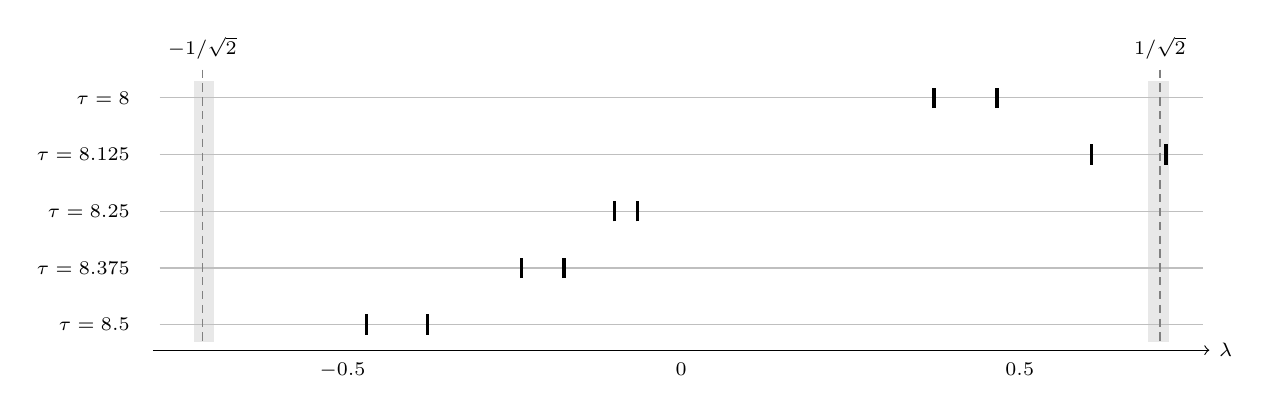
\begin{tikzpicture}[x=8.6cm,y=0.72cm]
  \fill[black!9] (0.69,0.3) rectangle (0.72,-4.3);
  \fill[black!9] (-0.72,0.3) rectangle (-0.69,-4.3);
  \foreach \y/\t/\a/\b in {0/8/0.373543/0.466256,-1/8.125/0.605497/0.716075,-2/8.25/-0.098190/-0.064436,-3/8.375/-0.236090/-0.172944,-4/8.5/-0.464887/-0.374640} {
    \draw[gray!50] (-0.77,\y) -- (0.77,\y);
    \node[font=\scriptsize,anchor=east] at (-0.8,\y) {$\tau=\t$};
    \draw[very thick] (\a,{\y-0.18}) -- (\a,{\y+0.18});
    \draw[very thick] (\b,{\y-0.18}) -- (\b,{\y+0.18});
  }
  \draw[densely dashed,gray] (0.707107,0.5) -- (0.707107,-4.3);
  \draw[densely dashed,gray] (-0.707107,0.5) -- (-0.707107,-4.3);
  \node[font=\scriptsize,anchor=south] at (0.707107,0.5) {$1/\sqrt2$};
  \node[font=\scriptsize,anchor=south] at (-0.707107,0.5) {$-1/\sqrt2$};
  \foreach \x in {-0.5,0,0.5}
    \node[font=\scriptsize,anchor=north] at (\x,-4.5) {$\x$};
  \draw[->] (-0.78,-4.45) -- (0.78,-4.45) node[right,font=\scriptsize] {$\lambda$};
\end{tikzpicture}
\caption{Fractional-scale dependence: each row shows all eigenvalues with
$0.05<|\lambda|<0.72$; shading marks $0.69<|\lambda|<0.72$.
The selection is not a continuation of fixed branches: the last three
scales also have a positive eigenvalue outside the window, at $0.7478$,
$0.7836$ and $0.7860$. Thus neither displayed signs nor guard-band
emptiness is uniform in $\tau$. Gauss--Legendre and Clenshaw--Curtis
values agree to $10^{-10}$; these are ordinary-precision samples from
\texttt{anc/verify\_phase\_dependence.py}, not certified boundary limits.}
\label{fig:phase-dependence}
\end{figure}

